\documentclass[convert]{standalone}

\usepackage{tikz}
\usetikzlibrary{shapes}
\begin{document}
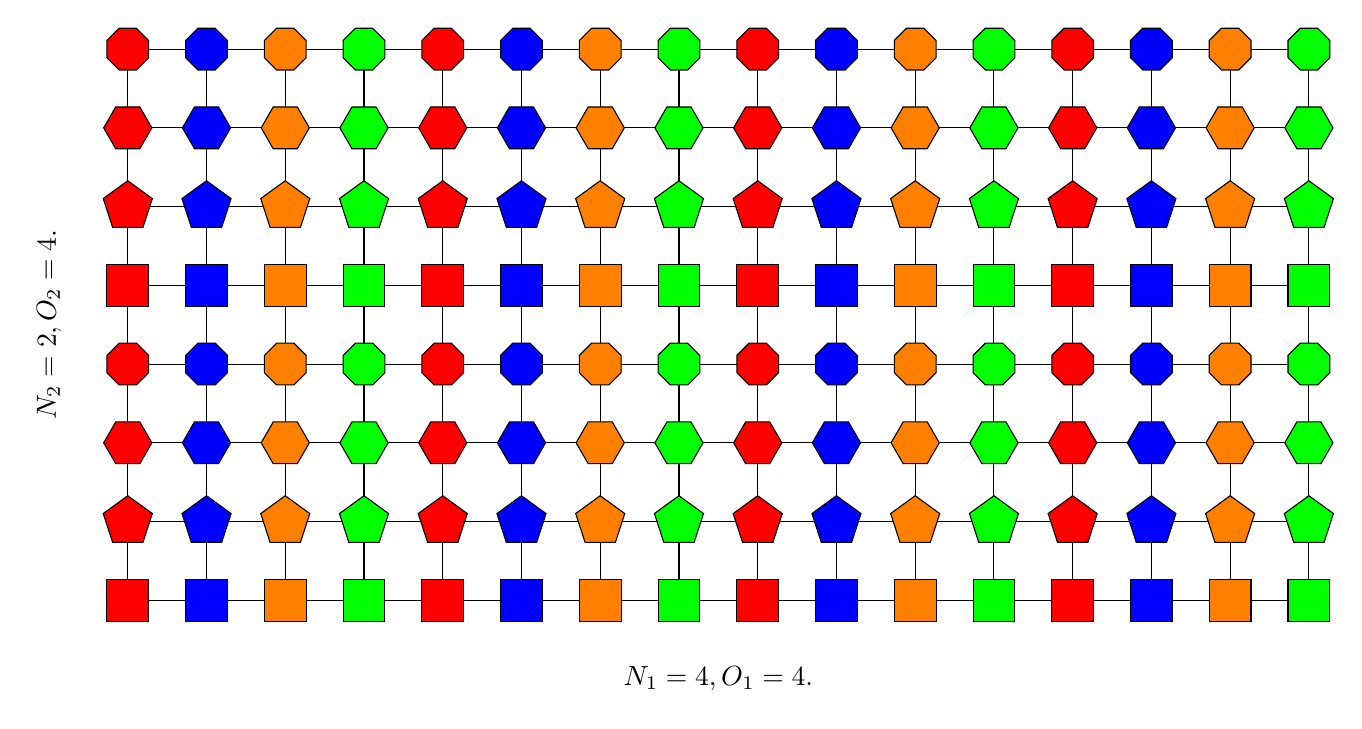
\begin{tikzpicture}
    \tikzstyle{o11} = [draw, fill=red, scale=1.6]
    \tikzstyle{o12} = [draw, fill=blue, scale=1.6]
    \tikzstyle{o13} = [draw, fill=orange, scale=1.6]
    \tikzstyle{o14} = [draw, fill=green, scale=1.6]
    \tikzstyle{o21} = [regular polygon, regular polygon sides=4]
    \tikzstyle{o22} = [regular polygon, regular polygon sides=5]
    \tikzstyle{o23} = [regular polygon, regular polygon sides=6]
    \tikzstyle{o24} = [regular polygon, regular polygon sides=8]
    \draw (0, 0) grid (15, 7);
    \foreach \nx in {0, 1, 2, 3}
    \foreach \ny in {0, 1}
    {
      \node at (\nx * 4, \ny * 4) [o11, o21] {};
      \node at (\nx * 4 + 1, \ny * 4) [o12, o21] {};
      \node at (\nx * 4 + 2, \ny * 4) [o13, o21] {};
      \node at (\nx * 4 + 3, \ny * 4) [o14, o21] {};
      \node at (\nx * 4, \ny * 4 + 1) [o11, o22] {};
      \node at (\nx * 4 + 1, \ny * 4 + 1) [o12, o22] {};
      \node at (\nx * 4 + 2, \ny * 4 + 1) [o13, o22] {};
      \node at (\nx * 4 + 3, \ny * 4 + 1) [o14, o22] {};
      \node at (\nx * 4, \ny * 4 + 2) [o11, o23] {};
      \node at (\nx * 4 + 1, \ny * 4 + 2) [o12, o23] {};
      \node at (\nx * 4 + 2, \ny * 4 + 2) [o13, o23] {};
      \node at (\nx * 4 + 3, \ny * 4 + 2) [o14, o23] {};
      \node at (\nx * 4, \ny * 4 + 3) [o11, o24] {};
      \node at (\nx * 4 + 1, \ny * 4 + 3) [o12, o24] {};
      \node at (\nx * 4 + 2, \ny * 4 + 3) [o13, o24] {};
      \node at (\nx * 4 + 3, \ny * 4 + 3) [o14, o24] {};
    }
    \node at (7.5, -1) {$N_1 = 4, O_1 = 4.$};
    \node at (-1, 3.5)[rotate = 90] {$N_2 = 2, O_2 = 4.$};
\end{tikzpicture}
\end{document}

%%% Local Variables:
%%% mode: latex
%%% TeX-master: t
%%% End:
